\chapterimage{images/testing/usertesting.jpg}

\chapter{Testing in Android}

\section{The testing pyramid}
The Testing Pyramid, shown in Figure 2, illustrates how your app should include the three categories of tests: small, medium, and large:

\begin{figure}[h]
	\centering
	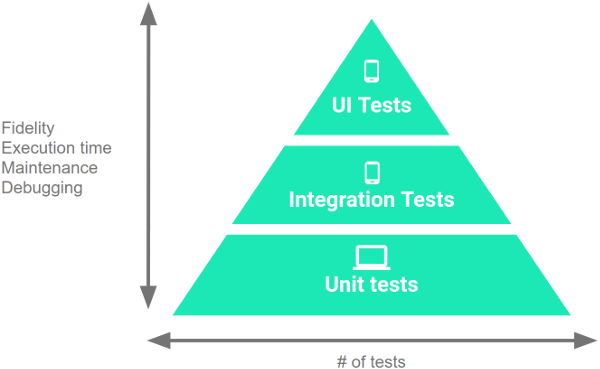
\includegraphics[width = 0.5\textwidth]{images/testing/pyramid}
	\caption{The Testing Pyramid, showing the three categories of tests that you should include in your app's test suite}
\end{figure}


Small tests are unit tests that you can run in isolation from production systems. They typically mock every major component and should run quickly on your machine.


Medium tests are integration tests that sit in between small tests and large tests. They integrate several components, and they run on emulators or real devices.


Large tests are integration and UI tests that run by completing a UI workflow. They ensure that key end-user tasks work as expected on emulators or real devices.


Although small tests are fast and focused, allowing you to address failures quickly, they're also low-fidelity and self-contained, making it difficult to have confidence that a passing test allows your app to work. You encounter the opposite set of tradeoffs when writing large tests.

Because of the different characteristics of each test category, you should include tests from each layer of the test pyramid. Although the proportion of tests for each category can vary based on your app's use cases, we generally recommend the following split among the categories: 70 percent small, 20 percent medium, and 10 percent large.

\section{Unit tests}
Unit tests are the fundamental tests in your app testing strategy. By creating and running unit tests against your code, you can easily verify that the logic of individual units is correct. Running unit tests after every build helps you to quickly catch and fix software regressions introduced by code changes to your app.

In your Android Studio project, you must store the source files for local unit tests at
\texttt{module-name/src/test/java/}. 
 
 This directory already exists when you create a new project.
 
 Your local unit test class should be written as a JUnit 4 test class. JUnit is the most popular and widely-used unit testing framework for Java. 

You also need to configure the testing dependencies for your project to use the standard APIs provided by the JUnit 4 framework.

To create a basic JUnit 4 test class, create a Java class that contains one or more test methods. A test method begins with the @Test annotation and contains the code to exercise and verify a single functionality in the component that you want to test.

See the 2048 example where a Unit Test has been added for the business logic.

\section{Espresso}
Espresso automatically synchronizes your test actions with the user interface of your application. The framework also ensures that your activity is started before the tests run. It also let the test wait until all observed background activities have finished.

It is intended to test a single application but can also be used to test across applications. If used for testing outside your application, you can only perform black box testing, as you cannot access the classes outside of your application.

Espresso has basically three components:

\begin{enumerate}
	\item ViewMatchers - allows to find view in the current view hierarchy
	
	\item ViewActions - allows to perform actions on the views
	
	\item ViewAssertions - allows to assert state of a view
\end{enumerate}

\begin{android}
onView(ViewMatcher)       
.perform(ViewAction)     
.check(ViewAssertion);
\end{android}

If Espresso does not find a view via the ViewMatcher, it includes the whole view hierarchy into the error message. That is useful for analyzing the problem.

See the example in \href{https://github.com/googlesamples/android-testing}{The testing examples}


\subsection{ActivityTestRule}
he following section describes how to create a new Espresso test in the JUnit 4 style and use ActivityTestRule to reduce the amount of boilerplate code you need to write. By using ActivityTestRule, the testing framework launches the activity under test before each test method annotated with @Test and before any method annotated with @Before. The framework handles shutting down the activity after the test finishes and all methods annotated with @After are run.



\subsection{Hamcresting}
 The Hamcrest library provides us with common matchers and possibility to create custom matchers. Hamcrest provides a library of matcher objects (also known as constraints or predicates) allowing 'match' rules to be defined declaratively, to be used in other frameworks. Typical scenarios include testing frameworks, mocking libraries and UI validation rules.
 
 The base idea is that matcher is initialized with the expected values, which are compared against the actual object we are matching when invoking it.
 
 Among of the common matchers you can create your custom matchers using abstract class TypeSaveMatcher.class , with three methods to override:
 
 \begin{enumerate}
 	\item public boolean matchesSafely() - matcher's logic,
 	\item protected void describeMismatchSafely Description 
 \end{enumerate}

To see this at work, refer to the \href{https://github.com/googlesamples/android-testing/tree/master/ui/espresso/CustomMatcherSample}{CustomMatcherSample}.

\section{Working with data adapters}
AdapterViews such as list, grids and spinners are different than the usual layouts (e.g. LinearLayout) because they don’t keep all their child elements in the view hierarchy. The main purpose of AdapterViews is to show large data sets on the screen efficiently, so they have to optimize memory use and performance by only maintaining a View object for data elements that currently fit inside the viewport.
All other elements exist only as the data set in the Adapter that is backing the AdapterView. With Espresso.onData(Matcher dataMatcher) you supply a Matcher that will try to match a row in the Adapter. If there is a successful match, Espresso will then bring that row onto the screen and into the view hierarchy so that you can perform actions and check assertions on its view as usual:

\begin{android}
onData(Matcher dataMatcher)
.perform(ViewAction action)
.check(ViewAssertion assert)
\end{android}


So how does the data matcher that you supply to onData() work? Basically, Espresso goes through the items in the Adapter backing your AdapterView one by one, and passes the result of Adapter.getItem(int position) to the Matcher.

See the \href{https://github.com/googlesamples/android-testing/tree/master/ui/espresso/DataAdapterSample}{Data Adapter sample for Espresso}

\subsubsection{The case of the RecyclerView}


At first it might seem like the same method should be applied to a RecyclerView, as it also uses adapters to hold data and reuses a small amount of View objects to display that data on the screen. Unfortunately, RecyclerView does not inherit from AdapterView (it’s a direct subclass of ViewGroup instead), so you can’t use onData with it.
Instead, you should use one of the RecyclerViewActions methods to scroll the RecyclerView to the desired item and perform a ViewAction on it (using a ViewHolder matcher or position):

\begin{android}
onView(withId(R.id.myRecyclerView))
.perform(
RecyclerViewActions.actionOnItemAtPosition(0, click())
);
\end{android}

See the \href{https://github.com/googlesamples/android-testing/tree/master/ui/espresso/RecyclerViewSample}{RecyclerViewSample }

\subsection{Espresso UI recorder}
Android Studio provides an Run ▸ Record Espresso Test menu entry which allows you to record the interaction with your application and create a Espresso test from it.
